\documentclass{article}
\usepackage{amsmath}
\usepackage{graphicx}
\title{ IVP Analytic vs. Numerical Solution }

\begin{document}

\maketitle

\section{Problem}

To compare a NOAA's analytyic solution, Nicolksy 2018 Analytic, and a finite volume numerical solutions of $\eta$ of the following two shallow water problems:

\subsection {A zero initial velocity N wave (Catalina 1)}

\[
\begin{aligned}
\eta_0(x) = 0.006*e^{-0.4444(x-4.129)^2} - 0.018e^{-4(x-1.6384)} \\
u_0(x) = 0 \\
h = 0.1x \\
m = \infty  \\
\end{aligned}
\]

\subsection{An N wave with initial velocity (Catalina 1 with initial velocity)}

\[
\begin{aligned}
\eta_0(x) = 0.006*e^{-0.4444(x-4.129)^2} - 0.018e^{-4(x-1.6384)} \\
u_0(x) = \eta_0(x)/\sqrt{x} \\
h = 0.1x \\
m = \infty  \\
\end{aligned}
\]

In other words, a Gaussian initial wave with no initial velocity, and a plane-inclined shape ($y^\infty$). This reduces to a 1-1 SWE. We can reproduce this with a different slope and initial conditions easily.

\section{Setup}

Statistical comparison was done on an equally spaced grid of 1000 points in time on [0,3] and at 1000 points in x on [-2.5, 6.5]


\subsection{Numerical}

I set Deny's Catalina 1 "runwave.m" with the initial conditions. The following displays eta in the $(x,t)$ plane

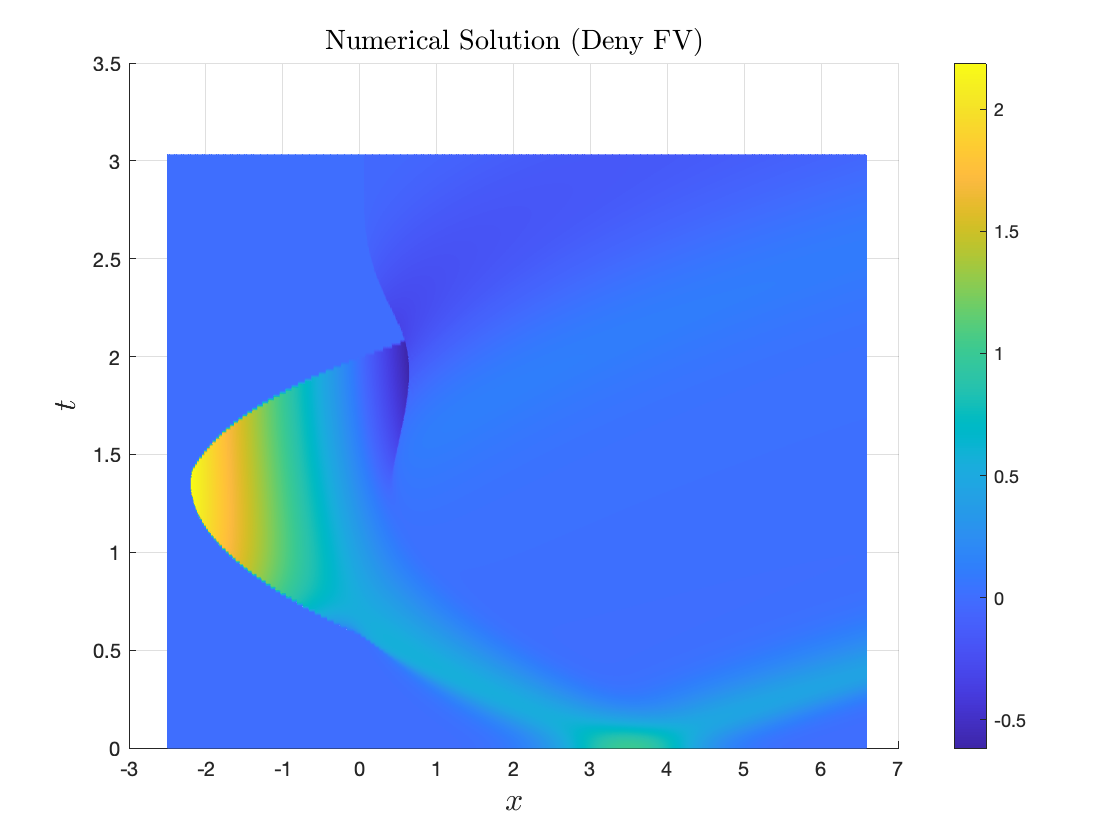
\includegraphics[width=\linewidth]{num.png} 


\subsection{Anaylytic}

Chebfun was used to calculate the Hankel transform solution to the CG transform on a grid in $(s,\lambda)$ then CG transform to $(x,t)$

\noindent The following figure shows the a grid in $(s,\lambda)$ transformed to $(x,t)$

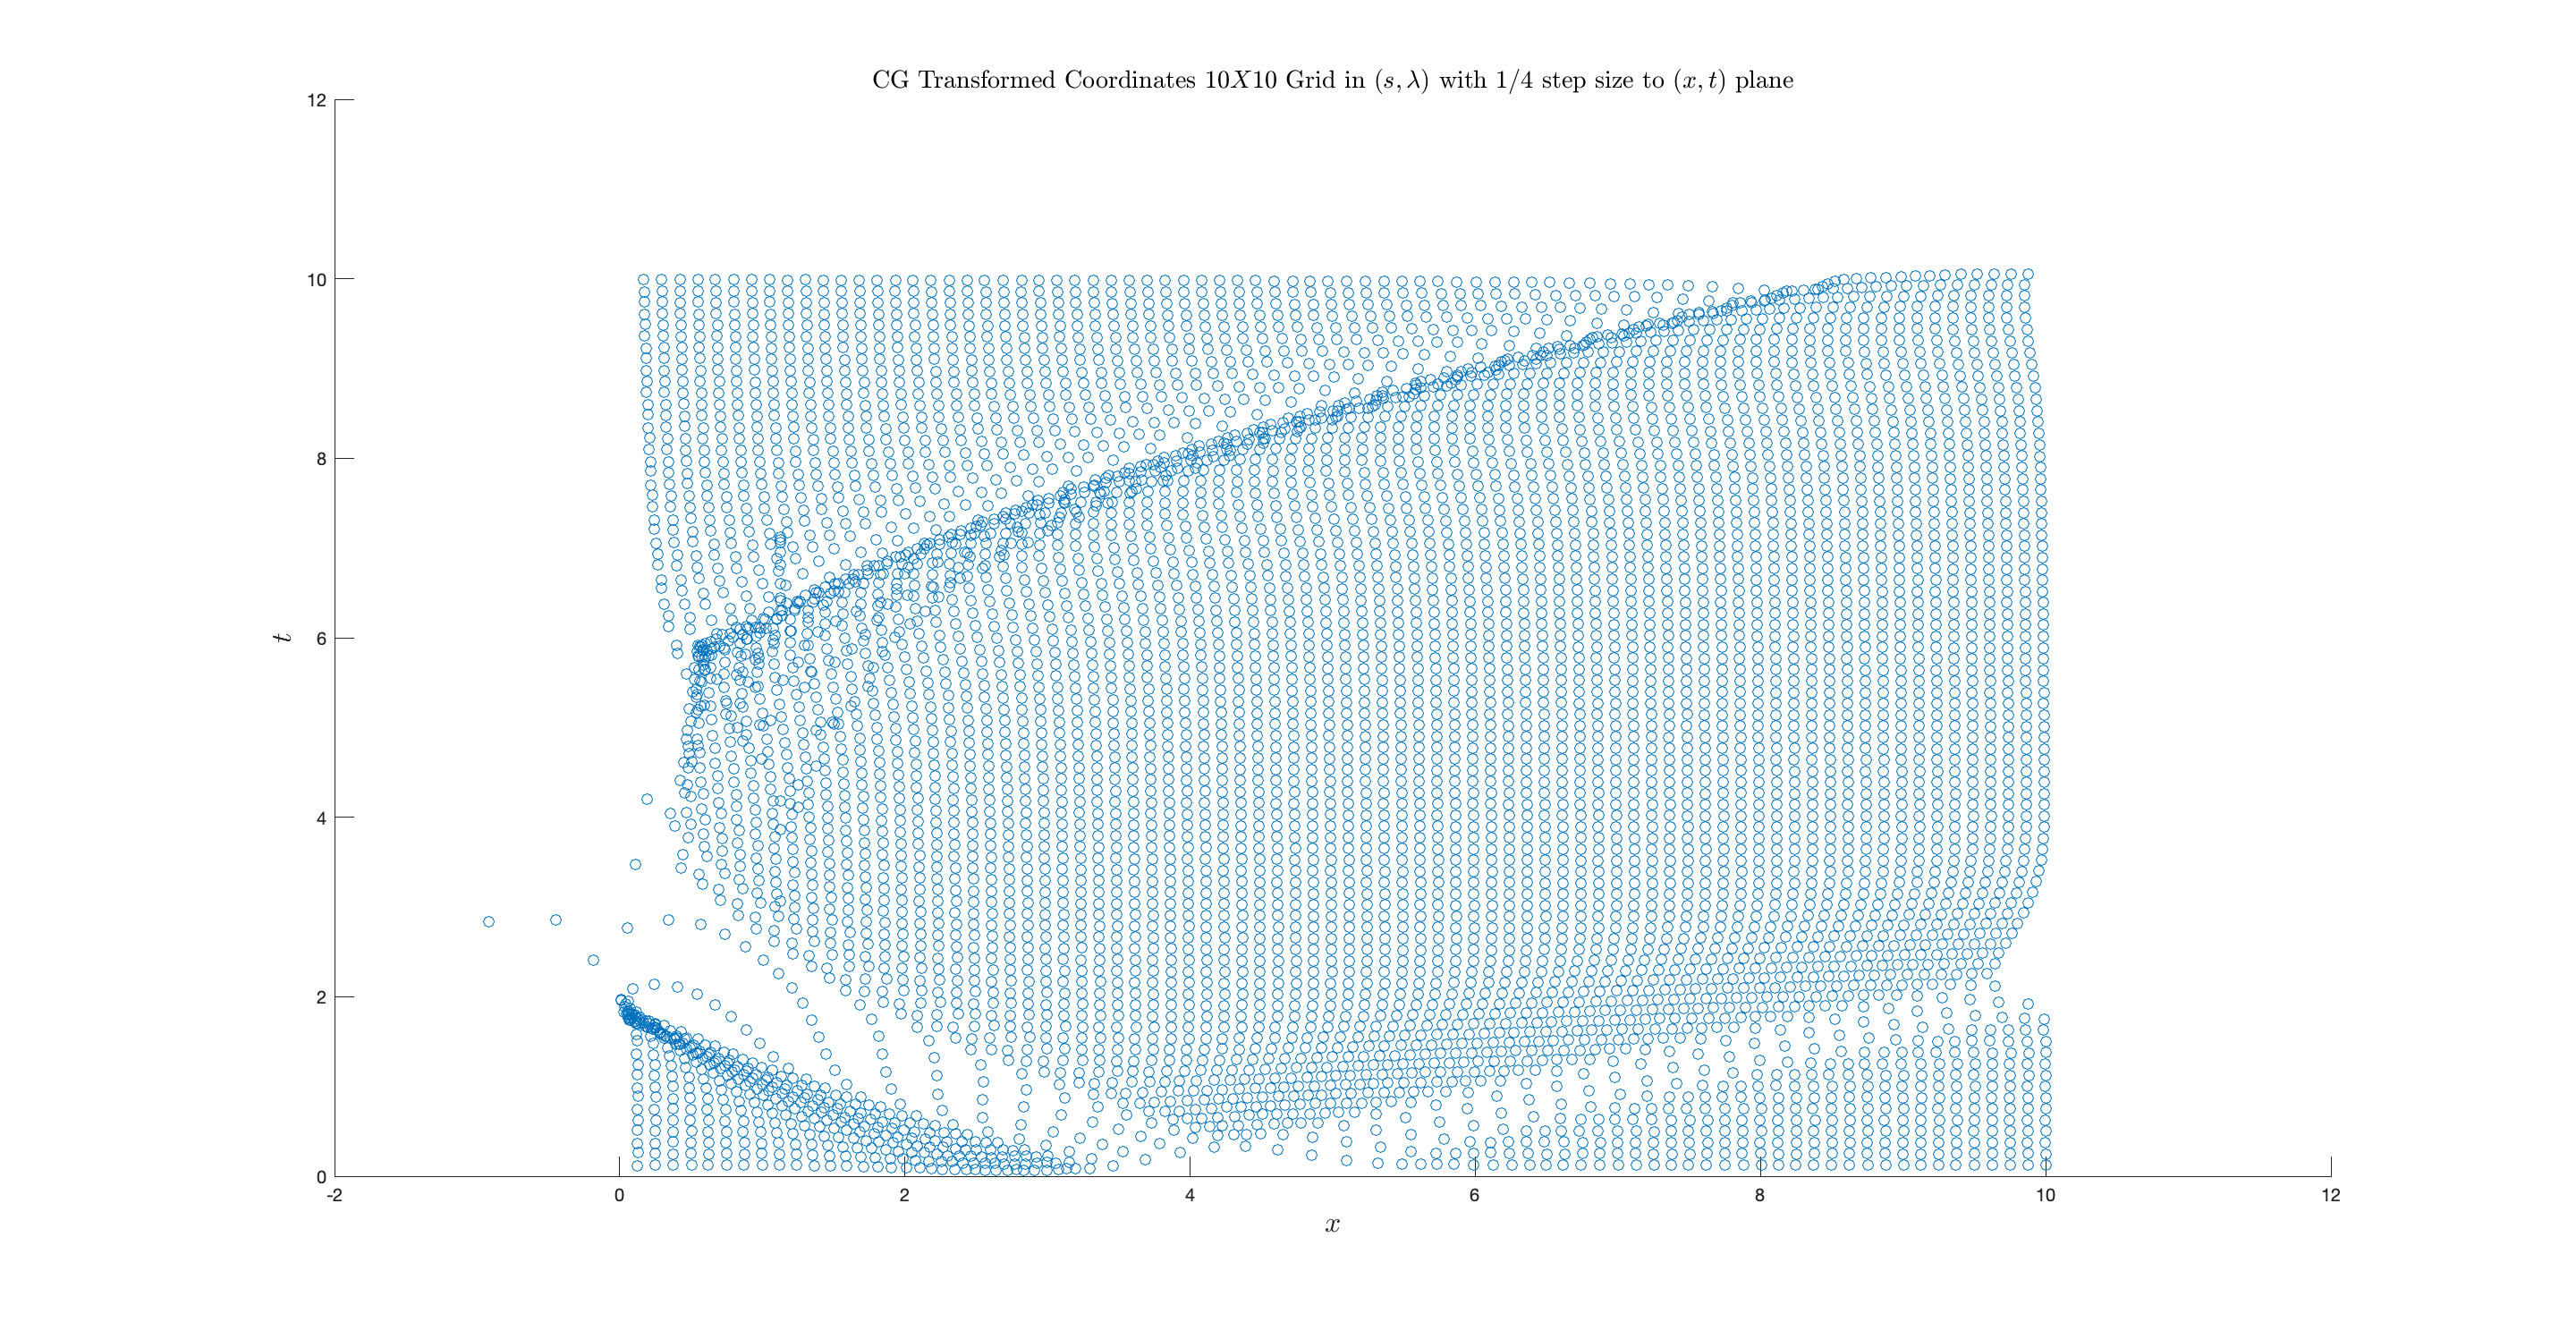
\includegraphics[width=\linewidth]{images/scatter.png} 

\noindent Note the distinct non-linear nature caused by the $-u^2$ of $\eta$

\noindent The analytical solution of $\eta$ was computed using formulas in Nicolsky (2018)

\[
\begin{aligned}
\psi (s, \lambda ) = \int_{0}^\infty (a(k)cos(\beta k \lambda)+b(k)sin(\beta k \lambda)) J_0(2 k \sqrt s ) dk\\
\varphi (s, \lambda ) =  s^{-1/2} \int_{0}^\infty (a(k)sin(\beta k \lambda)+b(k)cos(\beta k \lambda)) J_1(2 k \sqrt s )dk \\
\end{aligned}
\]

where

\[
\begin{aligned}
a(k) = 2k \int_{0}^\infty \psi(s*,0) J_0(2 k \sqrt {s*})ds*\\
b(k) = 2k \int_{0}^\infty \varphi(s*,0) s*^{1/2} J_1(2 k \sqrt {s*})ds*\\
\end{aligned}
\]

and the projection of $\varphi$ and $\psi$ onto $\lambda = 0$ were computed via a first order taylor expansion. Note that these eqautions require $\eta_0^\prime(x) > -1$.  See Nicolsky for derivation.

\[
\begin{aligned}
\Phi (s,\lambda) = \begin{pmatrix}
\varphi(s,\lambda) \\
\psi(s,\lambda)
\end{pmatrix} \\
\Phi_0(x) =  \begin{pmatrix}
u_0(x) \\
\eta_0(x) + u_0^2(x)/2
\end{pmatrix} \\
\Phi_1 = \Phi_0 + u_0(u_0^\prime A D^{-1} B \Phi_0 - B \Phi_0 - A D^{-1} \Phi_0^\prime)
\end{aligned}
\]

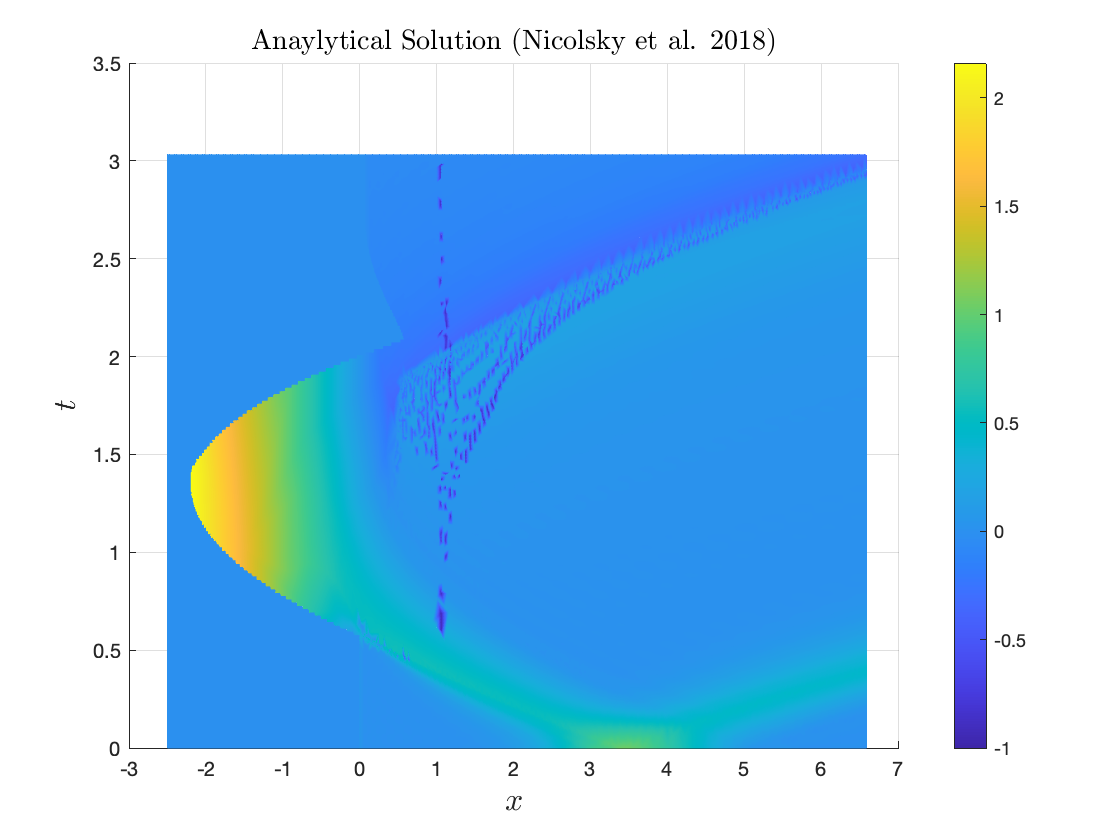
\includegraphics[width=\linewidth]{ana.png}

\section{Statistical Analysis}

This is the difference between the two ie. numerical - anaytical

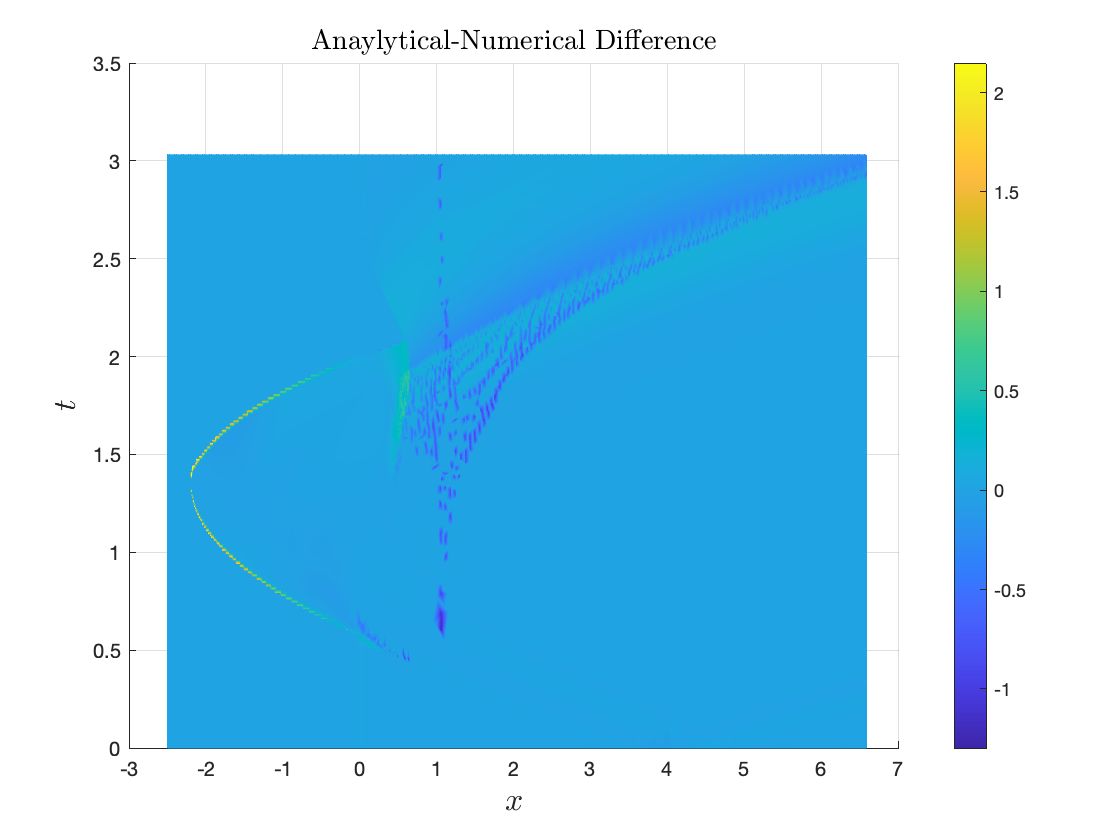
\includegraphics[width=\linewidth]{diff.png}

\noindent The following is the L2 norm at each value of t. The difference increases in a sporadic fashion at the beginning and end of run-up. The primary explaination for this is problems with the computation of the analytic solution.


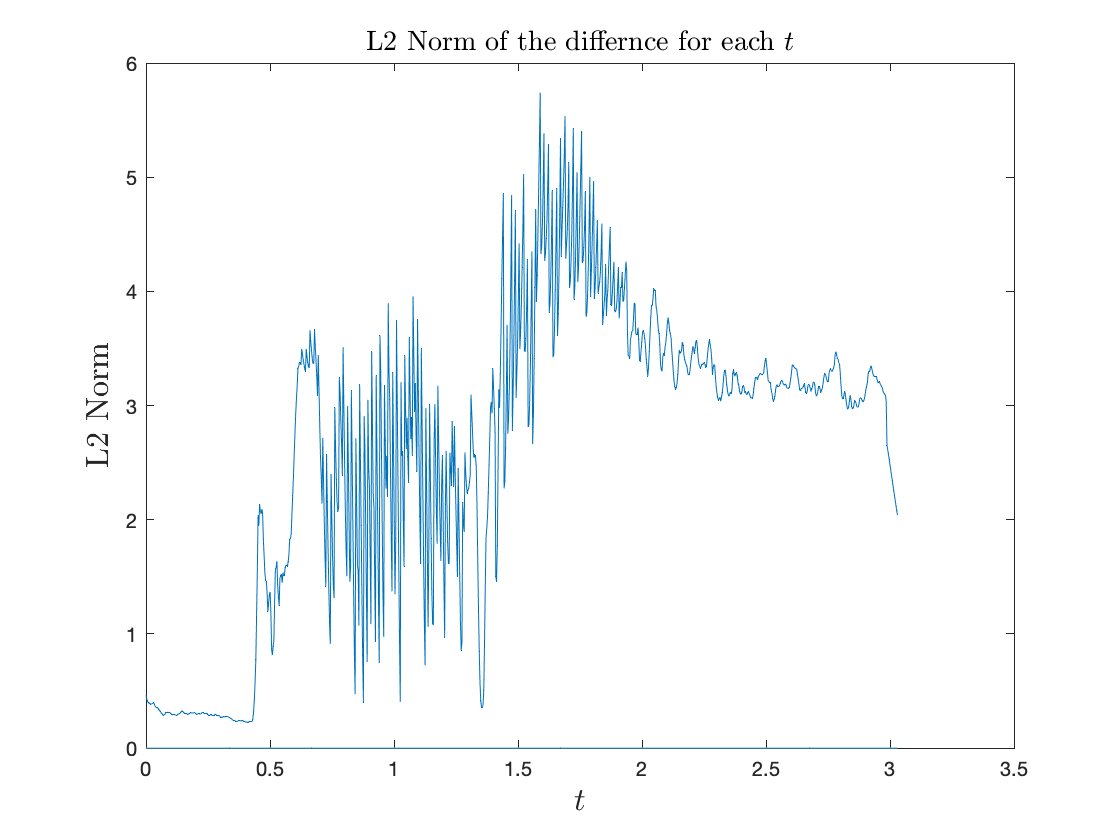
\includegraphics[width=\linewidth]{l2.png}

\section{Further Problems}

1. Analytic solution stability.

\noindent2. Comparison of the speed wasn't completed.

\noindent3. Different initial conditions.

\noindent4. NOAA anaytic solution.

\end{document}
